%=============================================================================
% CONFERENCE VERSION (6 pages, IEEE 2-column). Condensed from docs/paper/main.tex, which
% remains the full/extended version. Every numeric result traces to a CSV in ../../results/.
% Do NOT invent numbers.
%=============================================================================
\documentclass[conference]{IEEEtran}
\usepackage{graphicx}
\usepackage{booktabs}
\usepackage{amsmath}
\usepackage{amssymb}
\usepackage{amsthm}
\usepackage{url}
\usepackage[hidelinks]{hyperref}
\graphicspath{{../../results/}}
\newtheorem{proposition}{Proposition}

\begin{document}

\title{When Federated Log Anomaly Detection Silently Fails:\\
A Safety Map for Heterogeneous, Evolving Federations}

\author{\IEEEauthorblockN{Vansh Mundhra, Pinak Debnath, and Sankari M}
\IEEEauthorblockA{School of Computer Science and Engineering, Vellore Institute of Technology (VIT), Chennai, India\\
\{vansh.mundhra2023, pinak.debnath2023\}@vitstudent.ac.in,\ sankari.m@vit.ac.in}}

\maketitle

\begin{abstract}
Federated log anomaly detection is deployed exactly where logs cannot be centralized---banks,
healthcare, telecom, multi-tenant clouds---which run \emph{many different} log sources and add new
ones over time. Two recently reported properties (lightweight detectors are distribution-invariant;
their size is bounded) were, however, only ever validated where every client holds the \emph{same}
dataset. Placing HDFS and BGL clients in one federation over a merged vocabulary, we show these
properties break \emph{silently}: domain-blind range aggregation collapses on the tighter domain
(HDFS Length $F_1\,0.538\!\rightarrow\!0.000$), and a deep model catastrophically forgets an earlier
domain the moment a new one is onboarded ($0.70\!\rightarrow\!0.04$)---losing up to $99.97\%$ of
detection with no error or crash. We prove the collapse as a containment condition, map the safe and
unsafe regimes as a $2\times2$ over \{arrival pattern\}$\times$\{representation\}, and show the
forgetting is architecture-general (an LSTM and a Transformer both forget). The fixes cost almost
nothing---$48$ bytes, a replay buffer smaller than the model, Pareto-competitive with A-GEM---and we
distill the map into a summary-statistics-only auditor that \emph{predicts} these failures before
training, validated on $14$ of $15$ measured configurations. All results are from real runs on
commodity CPU.
\end{abstract}

\begin{IEEEkeywords}
Federated learning, log anomaly detection, data heterogeneity, catastrophic forgetting, continual learning.
\end{IEEEkeywords}

\section{Introduction}
System logs are the primary forensic record of large deployments, and flagging anomalous log
sequences is central to reliability and security~\cite{landauer2023survey}. As logs originate from
distributed, privacy-sensitive sources, centralizing them is often infeasible; federated
learning~\cite{mcmahan2017communication} keeps raw logs on premises and shares only model updates.
A recent study by Pustozerova \emph{et al.}~\cite{pustozerova2026lightweight} benchmarks
\emph{lightweight} statistical detectors against \emph{deep} ones (DeepLog~\cite{du2017deeplog})
under Federated Averaging (FedAvg), reporting two attractive properties: (C1) lightweight detectors
are approximately \emph{invariant to client distribution}, and (C2) their size is \emph{bounded by a
finite event vocabulary}.

\textbf{The gap.} That evaluation is \emph{homogeneous}: every client holds a slice of the
\emph{same} dataset (quantity skew). Real federations are \emph{domain-heterogeneous} (categorically
different log sources) and \emph{evolving} (new sources onboarded over time)---indeed the public
artifact of~\cite{pustozerova2026lightweight} ships \texttt{hdfs\_*} and \texttt{bgl\_*} configs but
no mixed one. The stakes are not academic: in exactly this regime detection collapses \emph{silently},
with no error or crash---up to $99.97\%$ of a detector's coverage lost (Sec.~\ref{sec:impact}), a
blind spot an operator never sees, yet one a few bytes of the right safeguard would prevent.

\textbf{Contributions.} (i) We place HDFS and BGL clients in one federation over a merged vocabulary
and show domain-blind range aggregation collapses on the tighter domain, which we \emph{prove} as a
containment condition, with a minimal domain-aware fix that restores it and routes with no oracle tag
($100\%$ accuracy). (ii) A controlled $2\times2$ map: simultaneous mixing is safe, but sequential
arrival catastrophically forgets \emph{iff} the representation shares a feature space---shown
\emph{architecture-general} across an LSTM and a Transformer. (iii) Mitigations (replay and EWC)
benchmarked against A-GEM, over which simple replay is Pareto-competitive. (iv) A deployable safety
auditor that predicts these failures from summary statistics alone, \emph{validated} on $14/15$
measured configurations. Every number traces to a result file.

\section{Method}
\textbf{Merged cross-domain vocabulary.} To let heterogeneous clients share one federation we build a
single global event space: each domain's parsed templates (via Drain~\cite{he2017drain}) form a
contiguous id block---HDFS owns $[0,33)$, BGL $[33,427)$---keyed \texttt{domain:id} so the two never
collide. A domain tag travels with each sequence for per-domain evaluation.

\textbf{Setup.} We use the HDFS and BGL benchmarks from Loghub~\cite{zhu2023loghub}. HDFS: $33$ event
types, $558{,}223$ normal / $16{,}838$ abnormal sequences, length $29\pm6$. BGL: $394$ types,
$37{,}823$ / $31{,}429$, length $69\pm747$. Following the reference, $1\%$ of each domain's normals
form the training pool (3 HDFS + 2 BGL clients); we report per-domain $F_1$ (anomaly is positive) as
mean\,$\pm$\,std over seeds $0$--$4$. All runs are CPU-only.

\textbf{Detectors.} \emph{Length} learns the $[\min,\max]$ normal length (domain-blind FedAvg =
global min/max); \emph{Known Events} learns the set of normal ids (FedAvg = set union);
\emph{DeepLog}~\cite{du2017deeplog} is a $2\times64$ LSTM predicting the next event from a length-$10$
window, anomalous if the true next event is not in the top-$9$. We support two DeepLog inputs: the
reference's raw scalar id, and a learned $16$-d embedding.

\textbf{Domain-aware fix.} Instead of one global range, domain-aware Length keeps a \emph{per-domain}
$[\min,\max]$ and routes a sequence to its domain's range. Because each domain owns a disjoint id
block, the domain is recoverable from the ids themselves (\emph{vocabulary-block routing}), so no
external tag is needed.

\section{When It Fails: The Safety Map}
\subsection{H1: range aggregation collapses (and we prove it)}
In the mixed federation, domain-blind Length on HDFS collapses to $F_1\approx0$: BGL's large spread
($69\pm747$) widens the shared global range until almost no HDFS sequence looks anomalous. Domain-aware
Length restores HDFS to $0.561\pm0.024$, its single-domain level (Table~\ref{tab:h1}). This is a direct
counterexample to C1 under domain skew. The collapse is structural, not a quirk of this pair:

\begin{proposition}[Range-aggregation collapse]\label{prop}
Let domain $a$ have normal-length range $[\underline{L}_a,\overline{L}_a]$ and anomaly-length support
$A_a$ disjoint from it (so a single-domain range detector attains recall $1$ on $A_a$). If some
co-training domain $b$ satisfies $A_a\subseteq[\underline{L}_b,\overline{L}_b]$, then domain-blind
Length attains recall $0$ on $a$, whereas domain-aware Length attains the single-domain recall.
\end{proposition}
\begin{proof}
The global range $[\min_d\underline{L}_d,\max_d\overline{L}_d]\supseteq[\underline{L}_b,\overline{L}_b]
\supseteq A_a$, so every $\ell\in A_a$ lies inside it and the flag predicate $\ell\notin[\cdot,\cdot]$
is false: no anomaly of $a$ is flagged, giving $F_1=0$. Domain-aware Length tests
$\ell\notin[\underline{L}_a,\overline{L}_a]$, true for all $\ell\in A_a$ by hypothesis. \qedhere
\end{proof}

\noindent The condition is \emph{relative}: a domain is safe only until a broader one joins. Adding
Hadoop (normal length up to $3{,}666>900$) to a four-domain federation flips BGL from widener to
victim (domain-blind Length $0.033\!\rightarrow\!0.001$), exactly as predicted, while HDFS is
unchanged and routing stays exact. \textbf{Tag-free routing} realizes the fix without a label:
vocabulary-block routing recovers the true domain of \emph{every} test sequence (accuracy
$1.000\pm0.000$) and reproduces the oracle-tag $F_1$ exactly (Table~\ref{tab:h1}); a conservative
no-inference variant instead collapses on HDFS. The effect is highly significant (paired
$t_4{=}47.4$, $p{=}1.2\times10^{-6}$).

\begin{table}[t]
\caption{H1: per-domain $F_1$ (mean$\pm$std, $5$ seeds), mixed federation. Vocabulary-block routing
equals oracle routing exactly. Source: \texttt{results/h1\_multiseed.csv}, \texttt{domain\_routing.csv}.}
\label{tab:h1}
\centering\small
\begin{tabular}{@{}lcc@{}}
\toprule
Method & HDFS $F_1$ & BGL $F_1$ \\
\midrule
Length, global (domain-blind)        & $0.000\pm0.000$ & $0.033\pm0.044$ \\
Length, domain-aware (ours, oracle tag) & $\mathbf{0.561\pm0.024}$ & $0.033\pm0.044$ \\
Length, domain-aware (vocab-block, no tag) & $\mathbf{0.561\pm0.024}$ & $0.033\pm0.044$ \\
\emph{HDFS single-domain Length} & \emph{0.538} & --- \\
\bottomrule
\end{tabular}
\end{table}

\subsection{H2/H3: simultaneous is safe, sequential forgets}
For the deep model the key axis is not mixing but \emph{arrival pattern combined with representation}
(Fig.~\ref{fig:map}). \emph{Simultaneous} mixed FedAvg does \emph{not} degrade DeepLog (HDFS drop
$+0.0002\pm0.0001$; BGL even improves), under both inputs. But under \emph{sequential} arrival the
embedding model \emph{catastrophically forgets} HDFS---$F_1\,0.70\!\rightarrow\!0.04$, forgetting
$0.665\pm0.003$---whereas the scalar input forgets nothing ($0.000$). A controlled scalar-vs-embedding
experiment isolates the cause: a \emph{shared feature space} across domains, not the aggregation
method ($p{=}1.2\times10^{-5}$). Separately, set-union Known Events never forgets but grows
$\times3.7$ per added domain, breaking C2 under evolution. The forgetting is also \emph{directional}:
the reverse order (broad domain first) does not forget ($-0.103$), so the dangerous case is onboarding
a broad-vocabulary domain after a narrow one.

\begin{figure}[t]
\centering
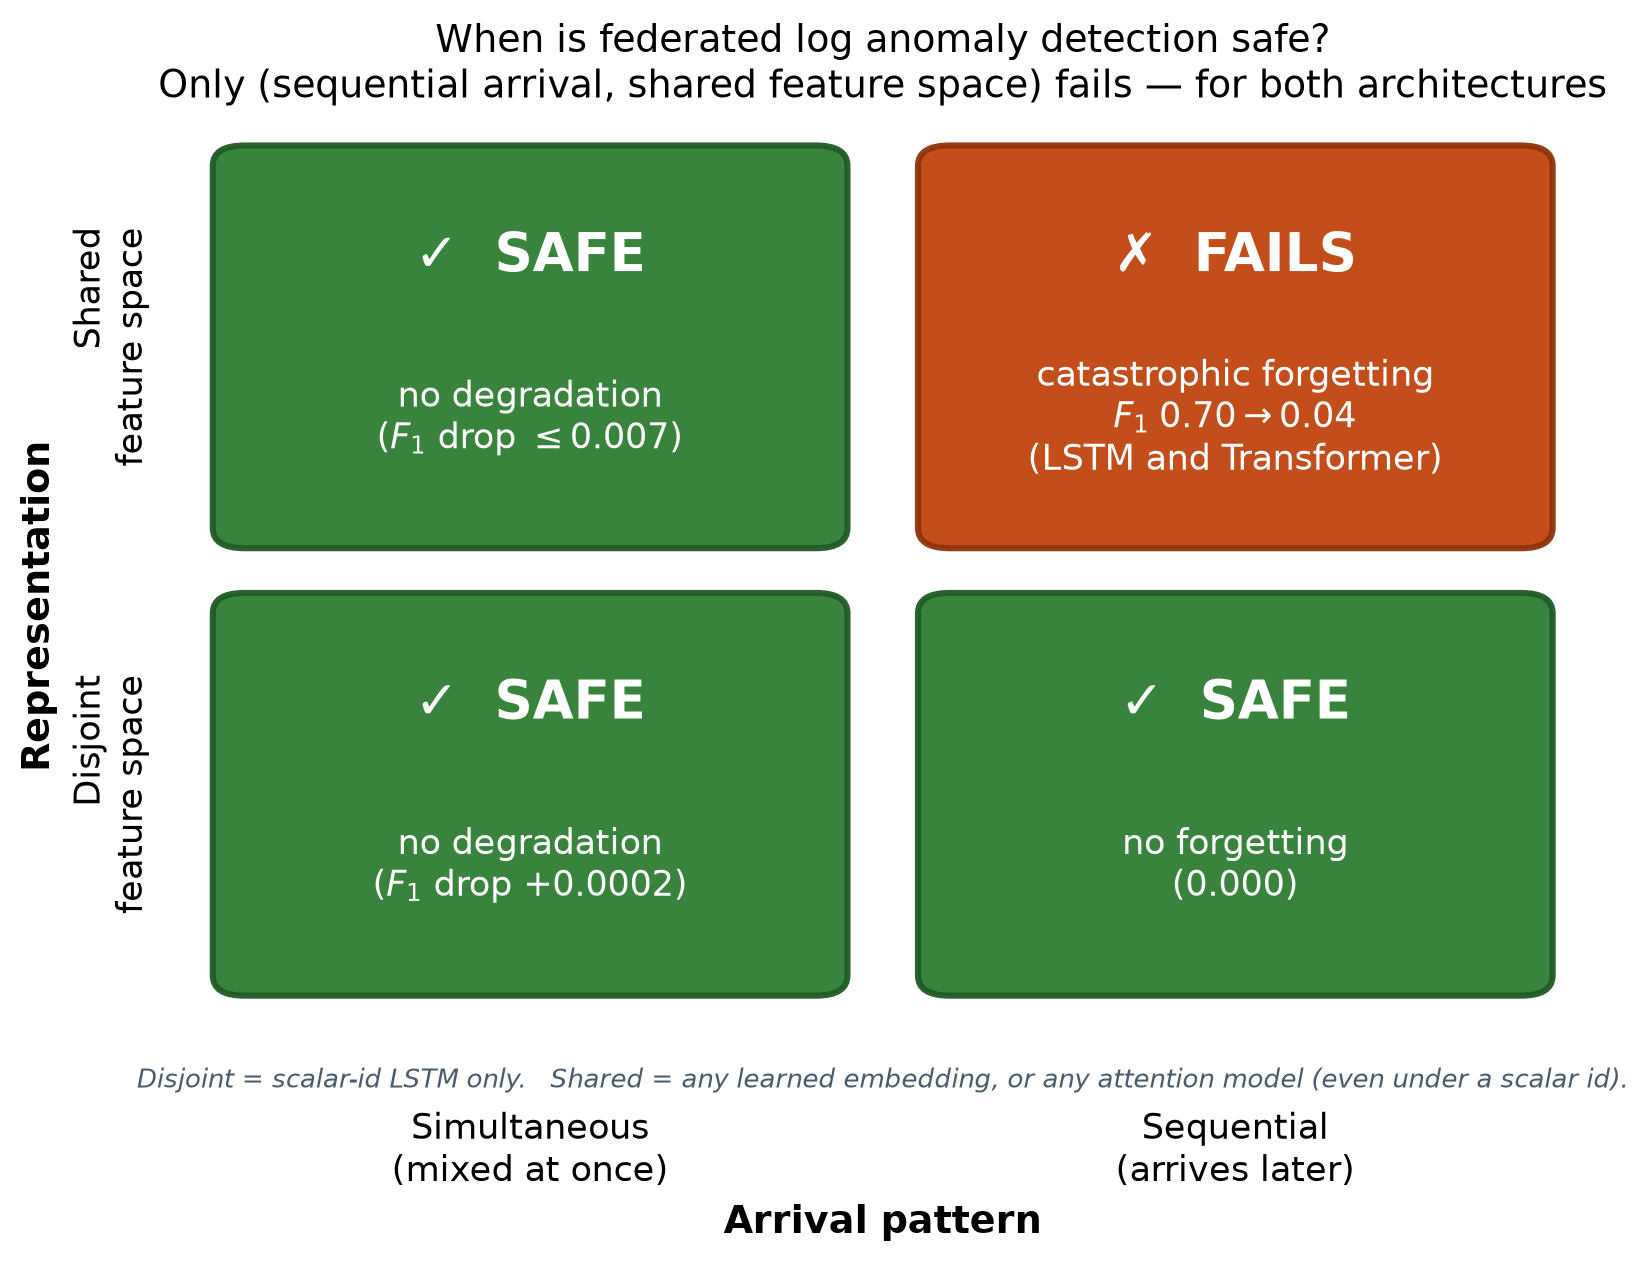
\includegraphics[width=0.84\columnwidth]{two_by_two_map.png}
\caption{The $2\times2$ safety map. Only \emph{(sequential, shared representation)} fails; the other
three regimes are safe. Confirmed for a Transformer as well (Fig.~\ref{fig:arch}).}
\label{fig:map}
\end{figure}

\subsection{The forgetting is architecture-general}
To test whether this is a DeepLog artifact, we replace the LSTM with a small self-attention Transformer
under the identical protocol (Fig.~\ref{fig:arch}). The map holds: simultaneous mixing is safe (HDFS
drop $\le0.02$), sequential arrival catastrophically forgets (scalar $0.636$, embedding $0.361$).
Tellingly, the Transformer forgets even under the \emph{scalar} input that leaves the LSTM immune,
because its input projection maps even a scalar id into a shared space. The operative cause is thus a
shared feature space---and modern/LLM-style encoders, which project inputs by construction, are
\emph{more} exposed, not less.

\begin{figure}[t]
\centering
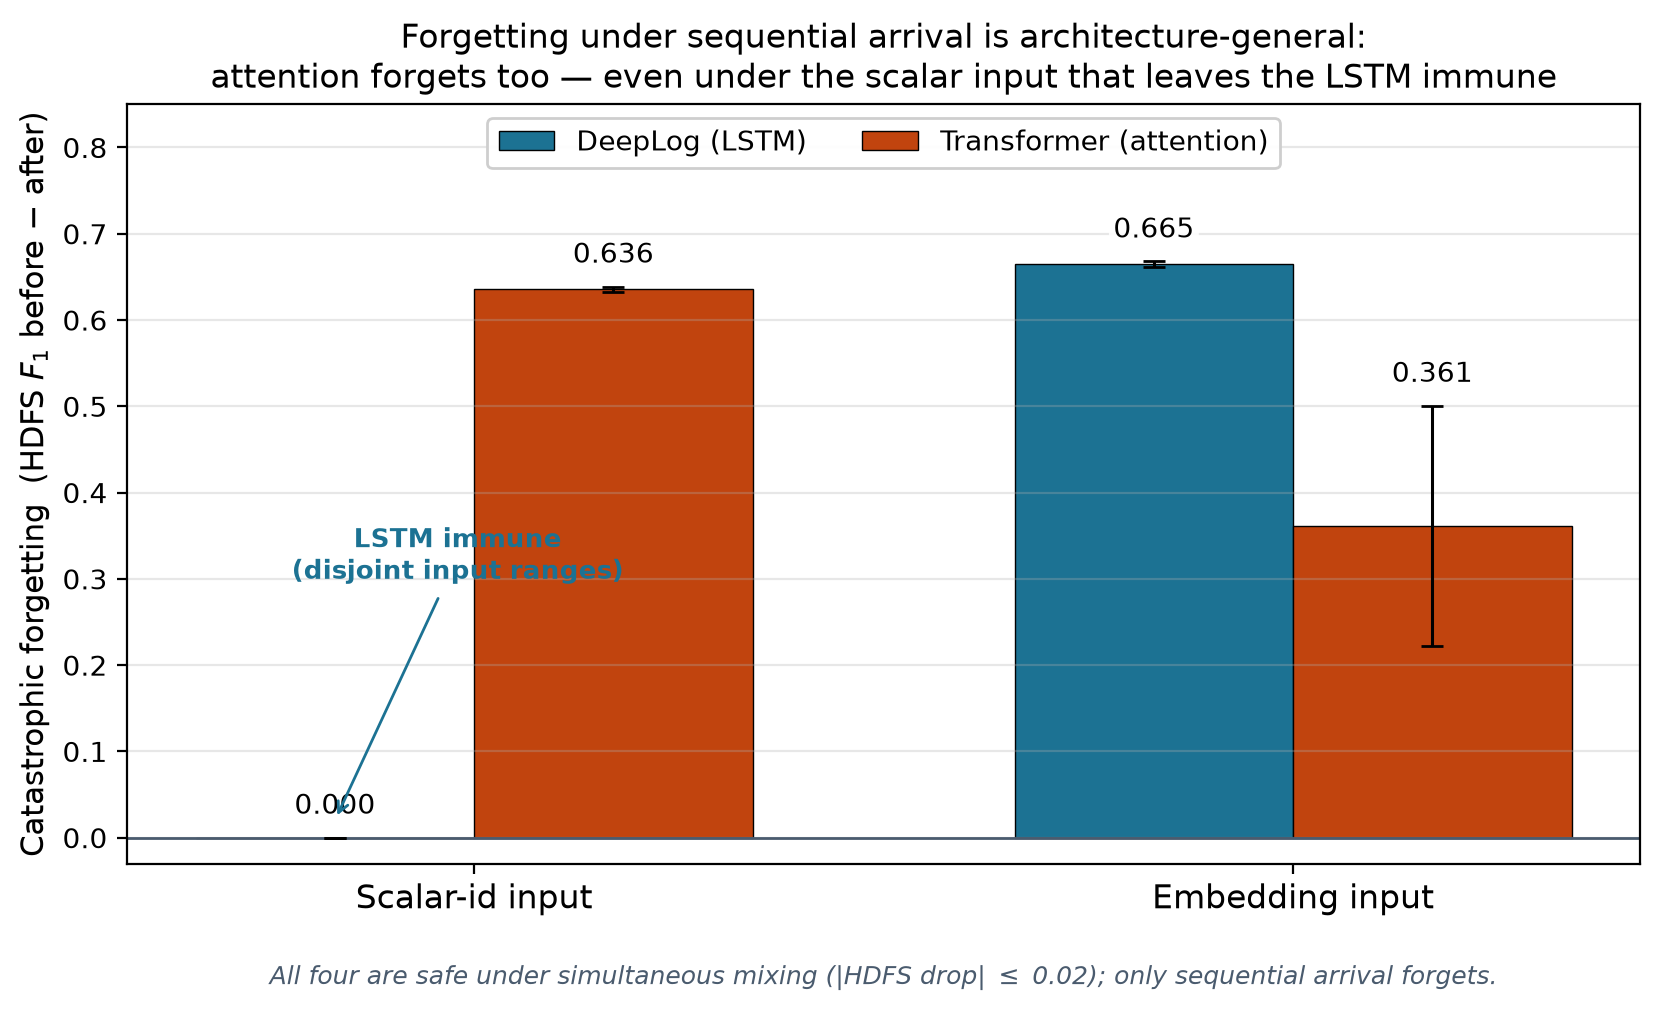
\includegraphics[width=0.96\columnwidth]{architecture_generality.png}
\caption{Forgetting is architecture-general. Of the four architecture$\times$input cells, only
DeepLog+scalar is immune; the Transformer forgets under \emph{both} inputs. All four are safe under
simultaneous mixing. Source: \texttt{results/transformer\_mechanism.csv}.}
\label{fig:arch}
\end{figure}

\section{Fixing It, Cheaply}
\subsection{Mitigation and a continual-learning baseline}
A diagnosis is actionable only if the failure is fixable. When the new domain arrives we retain a
small replay buffer of the earlier domain and train jointly; a $10\%$ buffer ($\approx558$ sequences)
cuts forgetting $0.665\!\rightarrow\!0.004$ while the new domain is still learned
(Table~\ref{tab:fix}). A memory-free EWC~\cite{kirkpatrick2017overcoming} alternative also works but
only at $\lambda{=}10^{8}$ (a six-order-of-magnitude search). Benchmarked against A-GEM~\cite{agem2019},
the standard episodic-memory method, at the \emph{same} memory budget, our plain replay matches it on
retention/forgetting and learns the new domain \emph{better} ($0.722$ vs.\ $0.657$)---A-GEM's gradient
projection over-constrains new-domain learning. Simple replay is thus Pareto-competitive with the
established toolkit; no exotic machinery is needed.

\begin{table}[t]
\caption{Mitigation comparison at a matched $10\%$ memory budget (embedding-DeepLog, sequential
HDFS$\rightarrow$BGL, mean$\pm$std, $3$ seeds). Sources:
\texttt{results/mitigation\_\{replay,agem,ewc\}.csv}.}
\label{tab:fix}
\centering\small
\begin{tabular}{@{}lcccc@{}}
\toprule
Method & Mem. & HDFS after & BGL after & Forgetting \\
\midrule
No defense              & ---   & $0.039$ & $0.642$ & $+0.665$ \\
EWC ($\lambda{=}10^{8}$) & none & $0.690$ & $\mathbf{0.752}$ & $+0.014$ \\
A-GEM~\cite{agem2019}   & $10\%$ & $0.698$ & $0.657$ & $+0.006$ \\
Replay (ours)           & $10\%$ & $\mathbf{0.700}$ & $0.722$ & $\mathbf{+0.004}$ \\
\bottomrule
\end{tabular}
\end{table}

\subsection{A validated safety auditor}
The guidances above are decision rules over quantities a federation knows \emph{before} training: each
domain's event-id block and length range, plus the intended arrival pattern and representation. We
compile the map into a pre-deployment auditor that takes only these per-client summary statistics---never
raw logs, preserving the federated privacy model---and returns which failures a planned federation will
hit and the prescribed fix. Crucially, we \emph{validate} it: run blind on every measured configuration
(two architectures $\times$ two inputs $\times$ arrival patterns, plus the lightweight collapse cases),
its verdict matches the observed outcome in $14$ of $15$ cases (Table~\ref{tab:audit}), including all
ten deep-model cells. The one error is a conservative false positive---the safe direction for a safety
check. Released as a CLI, it exits non-zero on a risky configuration and passes once a mitigation is
declared, gating a rollout in CI.

\begin{table}[t]
\caption{The auditor, run blind, predicts the measured outcome in $14/15$ configurations.
Source: \texttt{results/auditor\_validation.csv}.}
\label{tab:audit}
\centering\small
\begin{tabular}{@{}lcc@{}}
\toprule
Configuration group & Configs & Correct \\
\midrule
Deep-model forgetting (LSTM \& Transformer) & 10 & \textbf{10} \\
Lightweight range collapse (2- \& 3-domain)  & 5  & 4 \\
\midrule
Total & 15 & \textbf{14 ($93\%$)} \\
\bottomrule
\end{tabular}
\end{table}

\section{Why It Matters}\label{sec:impact}
The failures are \emph{silent and security-critical}: neither collapse nor forgetting raises an error
or crashes a service---the detector simply stops flagging anomalies for one domain while reporting
healthy operation for the rest. The magnitude is measured (Fig.~\ref{fig:impact}): domain-blind mixing
drops HDFS Length recall $0.369\!\rightarrow\!0.0001$, silently missing $6{,}209$ of $16{,}838$
anomalies ($99.97\%$ of coverage), and sequential onboarding erases $94.5\%$ of the deep model's
detection. A silent blind spot is more dangerous than an outage, because operators keep trusting a
system that has quietly stopped working---and \emph{extending} monitoring to a new source can
\emph{blind} monitoring of existing ones. Yet the safeguards cost almost nothing: per-domain ranges add
$48$ bytes, the replay buffer ($\approx126$\,KB) is smaller than the $347$\,KB model it protects, and
the auditor runs in $0.002$\,ms. Continuous \emph{effective} monitoring is also mandated (GDPR Art.~32,
HIPAA, PCI-DSS, NIS2); a detector that silently degrades on the next onboarding is a control gap the
auditor catches. There is no efficiency-versus-safety trade-off to agonize over---the safe
configuration is essentially free.

\begin{figure}[t]
\centering
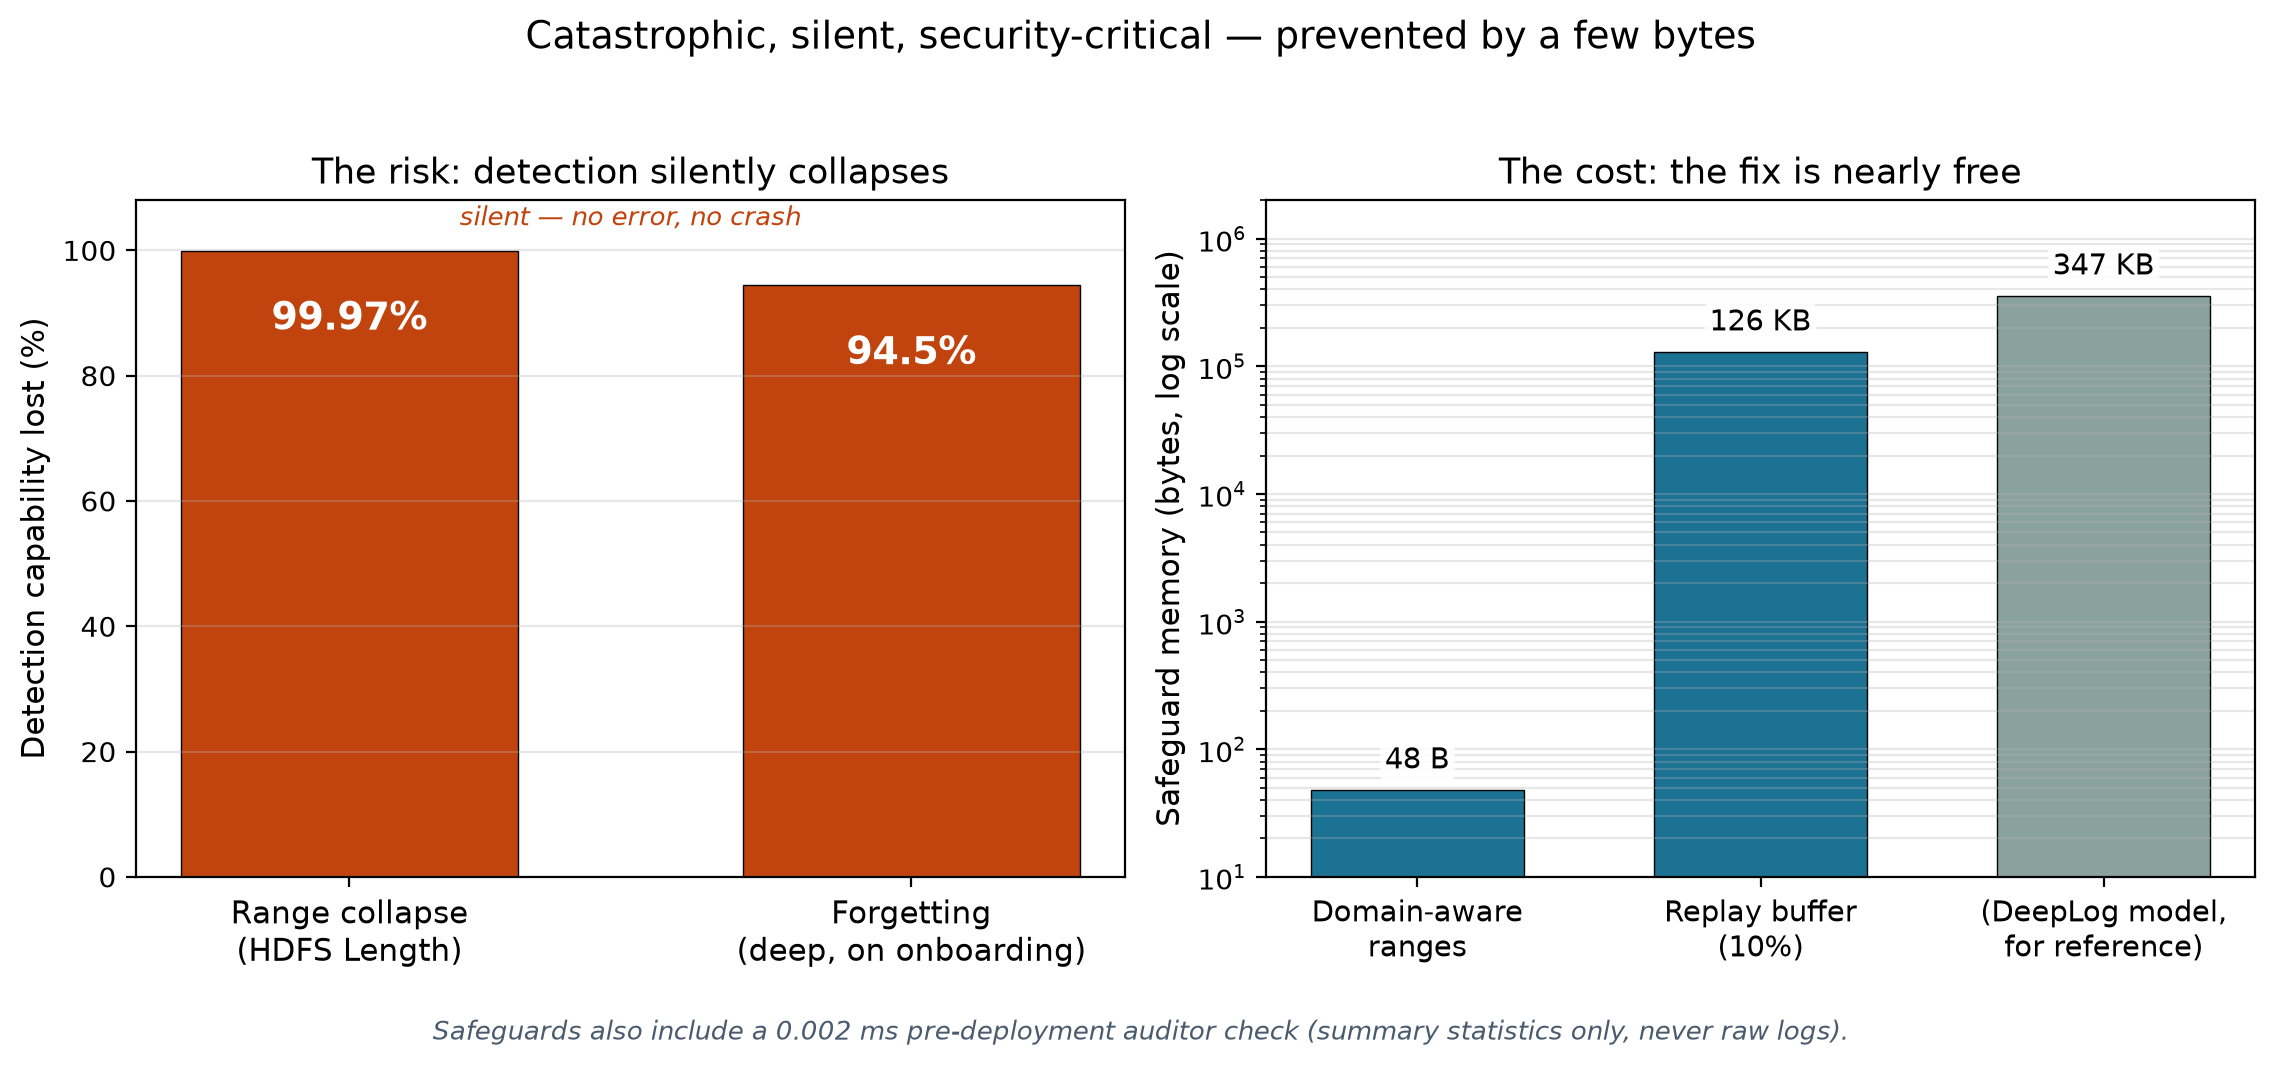
\includegraphics[width=\columnwidth]{impact_asymmetry.png}
\caption{Catastrophic, silent, security-critical---prevented by a few bytes. \emph{Left}: detection
lost when a failure fires. \emph{Right}: the safeguard's cost (log bytes), smaller than the model.
Source: \texttt{results/impact\_\{blindspot,overhead\}.csv}.}
\label{fig:impact}
\end{figure}

\section{Related Work}
Deep log detectors (DeepLog~\cite{du2017deeplog}, LogAnomaly~\cite{meng2019loganomaly}) and the
HDFS/BGL benchmarks~\cite{zhu2023loghub} are standard, but ask a question orthogonal to detector
design. FedAvg~\cite{mcmahan2017communication} and the heterogeneity survey of Kairouz \emph{et
al.}~\cite{kairouz2021advances} catalogue quantity/label/feature skew; the \emph{domain} skew we study
sits at the extreme of feature skew and is under-explored for logs. The closest work,
Pustozerova \emph{et al.}~\cite{pustozerova2026lightweight}, and a recent testbed
(FedLAD~\cite{fedlad2025}), keep every client on one dataset or provide infrastructure, but none
isolates the two claims under a single mixed-domain federation or identifies the input representation
as the lever governing forgetting. Sequential arrival is a continual-learning problem; EWC~\cite{kirkpatrick2017overcoming},
the continual survey~\cite{delange2022continual}, and A-GEM~\cite{agem2019} supply mitigations we
adopt and compare. Our contribution is the safety map, its proof, and a validated auditor for the
heterogeneous, evolving regime.

\section{Conclusion}
Two reported properties of federated log anomaly detection break in a heterogeneous, evolving
federation: range aggregation collapses (provably), and deep models forget under sequential arrival
into a shared representation---silently losing up to $99.97\%$ of detection, across two architectures
and up to four domains. The fixes are near-free and Pareto-competitive with the established toolkit,
and a validated, summary-statistics-only auditor predicts the failures before training. One limitation:
our federated DeepLog operates at $F_1\approx0.70$, not the reference's tuned $\sim0.93$ (a documented
scalar-input ceiling); the forgetting result is a \emph{relative} effect and unaffected. Future work:
alert-labelled sources (Thunderbird, Spirit) and automatic EWC-penalty selection.

\begin{thebibliography}{99}
\bibitem{landauer2023survey} M.~Landauer \emph{et al.}, ``Deep learning for anomaly detection in log
data: A survey,'' \emph{Mach. Learn. Appl.}, vol.~12, p.~100470, 2023.
\bibitem{mcmahan2017communication} B.~McMahan \emph{et al.}, ``Communication-efficient learning of
deep networks from decentralized data,'' in \emph{AISTATS}, 2017, pp.~1273--1282.
\bibitem{pustozerova2026lightweight} A.~Pustozerova \emph{et al.}, ``Lightweight techniques for
federated anomaly detection in log data,'' \emph{IEEE Trans. Rel.}, vol.~75, 2026.
\bibitem{du2017deeplog} M.~Du, F.~Li, G.~Zheng, and V.~Srikumar, ``DeepLog: Anomaly detection and
diagnosis from system logs through deep learning,'' in \emph{ACM CCS}, 2017, pp.~1285--1298.
\bibitem{meng2019loganomaly} W.~Meng \emph{et al.}, ``LogAnomaly: Unsupervised detection of sequential
and quantitative anomalies in unstructured logs,'' in \emph{IJCAI}, 2019, pp.~4739--4745.
\bibitem{he2017drain} P.~He, J.~Zhu, Z.~Zheng, and M.~R.~Lyu, ``Drain: An online log parsing approach
with fixed depth tree,'' in \emph{IEEE ICWS}, 2017, pp.~33--40.
\bibitem{zhu2023loghub} J.~Zhu \emph{et al.}, ``Loghub: A large collection of system log datasets for
AI-driven log analytics,'' in \emph{IEEE ISSRE}, 2023.
\bibitem{kairouz2021advances} P.~Kairouz \emph{et al.}, ``Advances and open problems in federated
learning,'' \emph{Found. Trends Mach. Learn.}, vol.~14, no.~1--2, pp.~1--210, 2021.
\bibitem{fedlad2025} Y.~Liao \emph{et al.}, ``FedLAD: A modular and adaptive testbed for federated log
anomaly detection,'' \emph{arXiv:2512.08277}, 2025.
\bibitem{kirkpatrick2017overcoming} J.~Kirkpatrick \emph{et al.}, ``Overcoming catastrophic forgetting
in neural networks,'' \emph{PNAS}, vol.~114, no.~13, pp.~3521--3526, 2017.
\bibitem{delange2022continual} M.~De~Lange \emph{et al.}, ``A continual learning survey: Defying
forgetting in classification tasks,'' \emph{IEEE TPAMI}, vol.~44, no.~7, pp.~3366--3385, 2022.
\bibitem{agem2019} A.~Chaudhry, M.~Ranzato, M.~Rohrbach, and M.~Elhoseiny, ``Efficient lifelong
learning with A-GEM,'' in \emph{ICLR}, 2019.
\end{thebibliography}

\end{document}
